\chapter{Arquitetura MVC}

    O sistema que se pretende implementar apresenta várias funcionalidades distintas, como a leitura de \textit{input}, a interpretação do mesmo, e acima de tudo, as alterações que este causa nas estruturas de dados centrais. Assim sendo, torna-se fundamental adotar um padrão arquitetural a fim de distribuir cada uma destas funcionalidades pelos vários módulos que este possua.

    Tendo em conta que foi referenciado nas aulas teóricas, escolhemos o padrão do MVC (\textit{Model-View-Controller}) como arquitetura do sistema, todavia a versão definida por nós permite a interação entre o \textit{Model} e a \textit{View}, visto que não faz muito sentido o \textit{Controller} ser um intermediário nas situações em que se limita a passar instruções sem sequer as alterar.

    \begin{figure}[hb!]
        \centering
        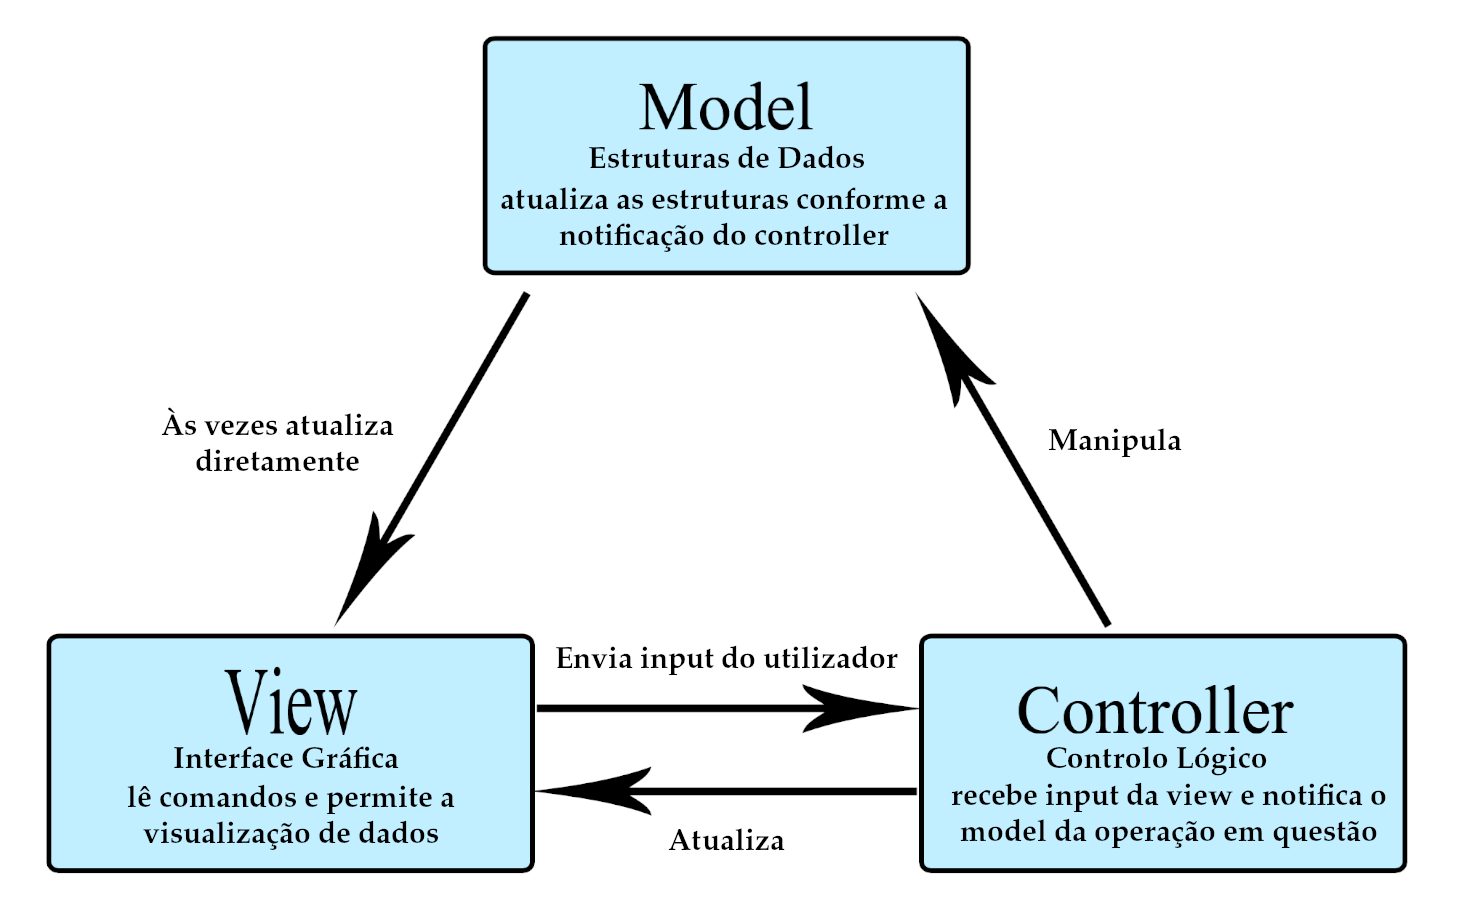
\includegraphics[width=0.7\textwidth]{imagens/8.png}
        \caption*{Figura 1. Arquitetura MVC}
    \end{figure}

    \vspace*{-15pt}
    \section{View}

    Um fator que julgamos ser bastante problemático diz respeito ao facto de a \textit{View} ler o \textit{input} e apresentar o \textit{output}, pois sendo estes dois tão distintos um do outro não há qualquer razão para estarem incluídos no mesmo código, como tal decidimos dividir a \textit{View} em duas classes designadas de \textit{Leitor} e \textit{Escritor,} que tal como o nome indica, são responsáveis por ler e escrever separadamente.

    Perante isto, o \textit{Leitor} comunica o \textit{input} ao \textit{Controlador,} enquanto que o \textit{Escritor} recebe dados do \textit{Controlador} e do \textit{Gestor} (Modelo) tendo em vista a apresentação dos mesmos.
    
    \begin{figure}[t]
        \centering
        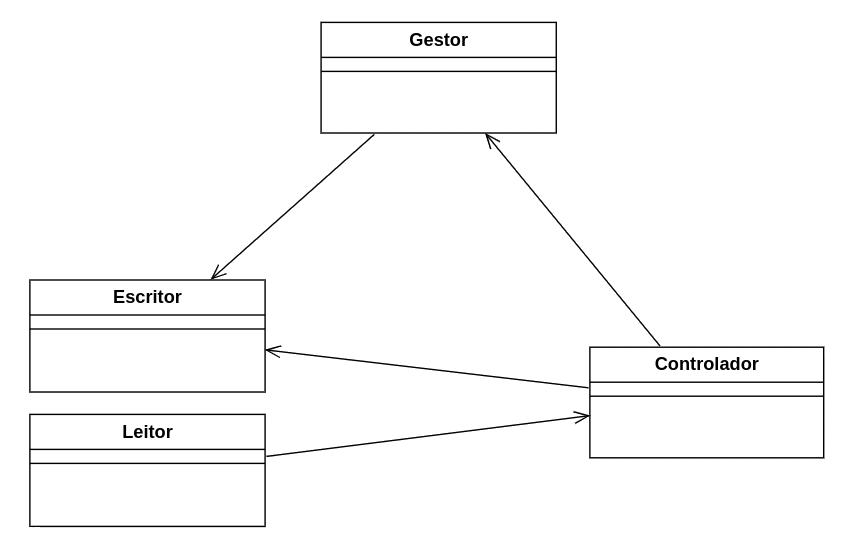
\includegraphics[width=0.7\textwidth]{imagens/7.png}
        \caption*{Figura 2. Padrão arquitetural final}
    \end{figure}
    
    Assim, com esta versão arquitetural fazemos uma clara distinção daquilo que são dados de \textit{input/output}, e consequentemente o \textit{Leitor} nem necessita de saber que o \textit{Escritor} existe e vice-versa, permitindo uma maior independência entre classes.

    \vspace{-5pt}
    \section{Controller}

    Conforme vai recebendo dados do \textit{Leitor,} o \textit{Controlador} tem a capacidade de fazer uma interpretação dos mesmos e informar o \textit{Gestor} de quais as operações que deve efetuar sobre as suas estruturas de dados, todavia o sistema dispõe de várias funcionalidades completamente distintas umas das outras, como a alteração de registos e cálculos estatísticos, portanto não há qualquer razão para o \textit{Controlador} saber todas as ordens que deve dar, até porque isso iria originar uma classe extremamente grande e complexa.

    \begin{figure}[hb!]
        \centering
        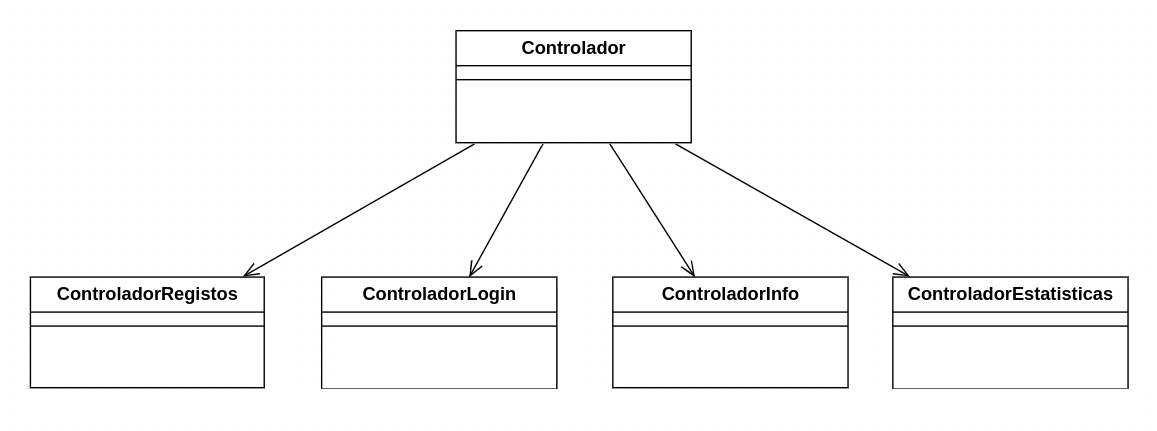
\includegraphics[width=0.8\textwidth]{imagens/10.png}
        \caption*{Figura 3. Divisão das funcionalidades por várias classes}
    \end{figure}

    Mais uma vez, a forma de resolver este problema passa pela distribuição e atribuição de tarefas a várias classes independentes entre si.

    \subsection{Controlador}

    Recebe uma mensagem do \textit{Leitor} e a partir daí faz uma interpretação de qual a funcionalidade requerida pelo utilizador, de seguida essa mesma mensagem é reenviada, juntamente com uma \textit{flag} a indicar a funcionalidade, para o respetivo controlador.
    
    \vspace*{-5pt}
    \subsection{ControladorRegistos}
    
    Ao receber a mensagem e \textit{flag} enviadas pelo \textit{Controlador,} sabe de que forma deve notificar o \textit{Gestor} sem que a mensagem tenha de voltar a ser interpretada, como se trata do controlador de registos, é natural que todas as suas notificações estejam relacionadas com a alteração das estruturas de dados presentes no \textit{Gestor.}

    \vspace*{-5pt}
    \subsection{ControladorLogin}
    
    Procede exatamente da mesma forma que o controlador anterior, contudo a notificação que envia diz respeito à autenticação de um utilizador a partir do seu \textit{email.}

    \vspace*{-5pt}
    \subsection{ControladorInfo}
    
    Notifica o \textit{Gestor} relativamente a pedidos de informação, sendo que mais tarde essa mesma informação é fornecida pelo \textit{Gestor} e reencaminhada para o \textit{Escritor.}

    \vspace*{-5pt}
    \subsection{ControladorEstatisticas}
    
    Notifica o \textit{Gestor} relativamente a questões estatísticas, tais como a listagem dos maiores vendedores/compradores/transportadoras. Ao receber uma notificação deste género, o \textit{Gestor} passa diretamente os dados ao \textit{Escritor} sem que haja qualquer reencaminhamento por parte deste controlador.

    \vspace*{-5pt}
    \subsection{Justificação}

    É certo que não era extremamente necessário criar novas classes para auxiliar o \textit{Controlador,} podendo este tratar de tudo, todavia esta implementação permite que o \textit{Controlador} apenas interprete mensagens enquanto que os restantes comunicam diretamente com o \textit{Gestor.}
    
    Assim, uma vez que o \textit{Controlador} não conhece o \textit{Gestor,} este funciona como uma espécie de fachada, visto que qualquer alteração dos demais controladores no máximo reflete-se no \textit{Controlador.}

    \newpage
    \section{Model}

    É dentro desta secção que estão incluídas as estruturas de dados que suportam por completo o correto funcionamento do sistema, como tal é aqui que a classe \textit{Gestor} opera conforme as notificações que recebe dos controladores.

    Uma vez que o \textit{Gestor} tem de salvaguardar os registos de objetos como utilizadores e artigos, este deve possuir estruturas de dados que permitam o acesso direto a um determinado objeto. Contudo, mais uma vez, não é correto implementar um \textit{Gestor} que possua coleções de objetos tão distintos.

    \begin{figure}[hb!]
        \centering
        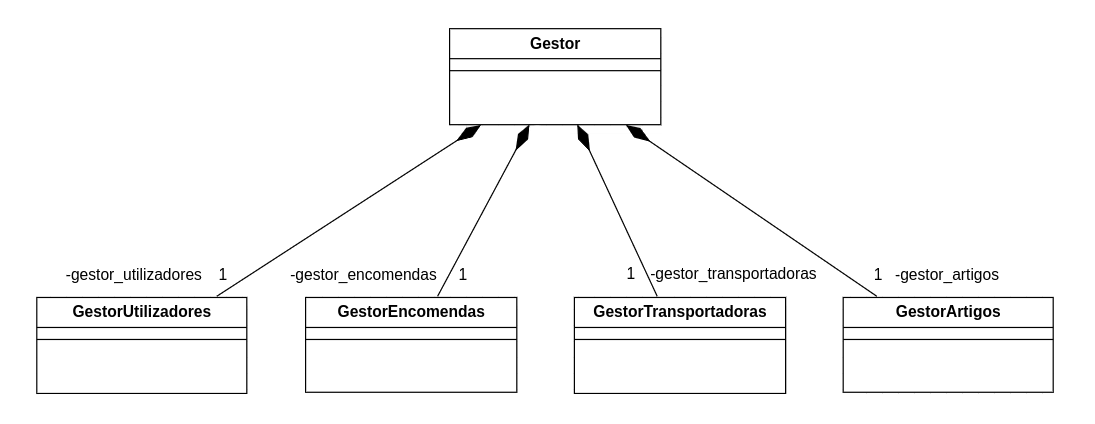
\includegraphics[width=0.85\textwidth]{imagens/6.png}
        \caption*{Figura 4. Distribuição das estruturas de dados pelas classes}
    \end{figure}

    Ao criar novas classes de gestores, nas quais cada uma controla e manipula as coleções referentes a um determinado objeto, o \textit{Gestor} pode alterar indiretamente os registos de qualquer coleção, bastando apenas invocar métodos dos demais gestores.

    Assim, tal como no caso anterior, o \textit{Gestor} funciona como uma fachada, visto que as alterações nos gestores propagam-se até ao \textit{Gestor} no prior dos casos.